% !TeX program = xelatex
%Document class article only supports 10pt, 11pt, and 12pt
\documentclass[a4paper,12pt,oneside,times,numbered,PageStyleI,custommargin]{PhDThesisPSnPDF}

% ******************************************************************************
% ******************************* Class Options ********************************
% ******************************************************************************

% `a4paper' (default): International A4 size paper, default option.
%
% `11pt' or `12pt'(default): Font Size.
%
% `oneside' (default) or `twoside': Printing double side (twoside) or single
% side. Printed copy of thesis should be typed on both sides of the paper.
%
% `print': Use `print' for print version with appropriate margins and page
% layout. Leaving the options field blank will activate Online version.
%
%
% *********************** Choosing the Fonts in Class Options ******************
%
% `times' : Times font with math support.
%
% `fourier': Utopia Font with Fourier Math font (Font has to be installed)
%            It's a free font.
%
% `customfont': Use `customfont' option in the document class and load the
% package in the preamble section below.
%
% default or leave empty: `Latin Modern' font will be loaded.
%
% ********************** Choosing the Bibliography style ***********************
%
% `authoryear': For author-year citation eg., Krishna (2013)
%
% `numbered': (Default Option) For numbered and sorted citation e.g., [1,5,2]
%
% `custombib': Define your own bibliography style in the preamble section below.
%              `\RequirePackage[square, sort, numbers, authoryear]{natbib}'.
%              This can be also used to load biblatex instead of natbib
%              (See Preamble)
%
% **************************** Choosing the Page Style *************************
%
% `(leave empty)': Page Numbers in footer (center). Blank Header.
%
% `PageStyleI': Chapter Name on Even Side (Left Even) in Header. Section Number
% and Section Name in Header on Odd Side (Right Odd). Use Header rule.
%
% `PageStyleII': Chapter Name on Even Side (Center) in Header. Section Number
% and Section Name in Header on Odd Side (Center). Use Header rule.
%
% `PageStyleIII': Chapter Name on Even Side (Left Even) in Header. Section Number
% and Section Name in Header on Odd Side (Right Odd). Don't use Header rule.

% ******************************************************************************
% ********************************** Preamble **********************************
% ******************************************************************************

% Contains packages and user-defined commands and settings

% ****************************** Custom Margin *********************************

% Add `custommargin' in the document class options to use this section
% Set {innerside margin / outerside margin / topmargin / bottom margin}  and
% other page dimensions
\ifsetCustomMargin
  \RequirePackage[left=37mm,right=30mm,top=35mm,bottom=30mm]{geometry}
  \setFancyHdr % To apply fancy header after geometry package is loaded
\fi

% Add spaces between paragraphs
\usepackage{parskip}
\setlength{\parskip}{1em} % 0.5em
% Ragged bottom avoids extra whitespaces between paragraphs
%\raggedbottom
% To remove the excess top spacing for enumeration, list and description
%\usepackage{enumitem}
%\setlist[enumerate,itemize,description]{topsep=0em}

% modification for figures caption
\usepackage[singlelinecheck=false, labelfont=bf]{caption} % make caption in bold
\usepackage{afterpage}

% Add underlines in publications
\usepackage{ulem}
\usepackage{amsmath}

% Change Chapter font size
\usepackage{sectsty,lmodern}

% Change font color
\usepackage{color}

% long tables for multiple pages in appendix
\usepackage{longtable}
% \usepackage{caption}
% The longtable documentation does give an example of how to produce a full width table:
% \setlength\LTleft{0pt}
% \setlength\LTright{0pt}
% \begin{longtable}{@{\extracolsep{\fill}}|c|c|c|@{}}

% ******************* Fonts (like different typewriter fonts etc.)*************

% Add `customfont' in the document class option to use this section

\ifsetCustomFont
  % Set your custom font here and use `customfont' in options. Leave empty to
  % load computer modern font (default LaTeX font).
  % \setmainfont{Georgia}
  \setromanfont{Times New Roman}
  \setsansfont{Arial}
  \setmonofont{Courier New}

\fi

% **************************** Custom Packages ********************************

% ************************* Algorithms and Pseudocode **************************

%\usepackage{algpseudocode}


% ********************Captions and Hyperreferencing / URL **********************

% Captions: This makes captions of figures use a boldfaced small font.
% \RequirePackage[small,bf]{caption}

\RequirePackage[labelsep=space,tableposition=top]{caption}
\renewcommand{\figurename}{Figure} %to support older versions of captions.sty


% *************************** Graphics and figures *****************************
%\usepackage{rotating}
%\usepackage{wrapfig}

% Uncomment the following two lines to force Latex to place the figure.
% Use [H] when including graphics. Note 'H' instead of 'h'
\usepackage{float}
%\restylefloat{figure}

% Subcaption package is also available in the sty folder you can use that by
% uncommenting the following line
% This is for people stuck with older versions of texlive
%\usepackage{sty/caption/subcaption}
\usepackage{subcaption}

%如果希望避免浮动体跨过 \section,可以使用 placeins 宏包。
\usepackage[section]{placeins}

% ********************************** Tables ************************************
\usepackage{booktabs} % For professional looking tables
\usepackage{multirow}

%\usepackage{multicol}
%\usepackage{longtable}
%\usepackage{tabularx}

% ************************ Formatting / Footnote *******************************

% Don't break enumeration (etc.) across pages in an ugly manner (default 10000)
%\clubpenalty=500
%\widowpenalty=500

%\usepackage[perpage]{footmisc} %Range of footnote options


% *************************** Bibliography  and References ********************

\usepackage{cleveref} %Referencing without need to explicitly state fig /table

% Add `custombib' in the document class option to use this section
\ifuseCustomBib
  \RequirePackage[square, sort, numbers, authoryear]{natbib} % CustomBib

% If you would like to use biblatex for your reference management, as opposed to
% the default `natbibpackage` pass the option `custombib` in the document
% class. Comment out the previous line to make sure you don't load the natbib
% package. Uncomment the following lines and specify the location of
% references.bib file. Do not omit the .bib extension from the filename.

% \RequirePackage[backend=biber, style=numeric-comp, citestyle=numeric, sorting=nty, natbib=true]{biblatex}
% \addbibresource{References/ref_1.bib}

\fi

% changes the default name `Bibliography` -> `References'
\renewcommand{\bibname}{References}

% ***************************** Better enumeration ****************************
\usepackage{enumitem}

% ******************************************************************************
% ************************* User Defined Commands ******************************
% ******************************************************************************

% *********** To change the name of Table of Contents / LOF and LOT ************

%\renewcommand{\contentsname}{My Table of Contents}
%\renewcommand{\listfigurename}{My List of Figures}
%\renewcommand{\listtablename}{My List of Tables}

% ********************** TOC depth and numbering depth *************************

\setcounter{secnumdepth}{2}
\setcounter{tocdepth}{2}


% ******************************* Nomenclature *********************************

% To change the name of the Nomenclature section, uncomment the following line

%\renewcommand{\nomname}{Symbols}


% ********************************* Appendix ***********************************

% The default value of both \appendixtocname and \appendixpagename is 
% `Appendices'.These names can all be changed via:

\renewcommand{\appendixtocname}{List of appendices}
%\renewcommand{\appendixname}{Appndx}

% ******************************* Publications *********************************

% To change the name of the Publications section, uncomment the following line
%\renewcommand{\pubname}{List of Publications}

% ********************************* Layout *************************************
% \usepackage{layout}
% \makeatletter
% \renewcommand*{\lay@value}[2]{%
% \strip@pt\dimexpr0.351459\dimexpr\csname#2\endcsname\relax\relax mm%
% }
% \makeatother

% ************************** Placeholder Text **********************************
\usepackage{lipsum}
\usepackage[math]{blindtext}

% *************************** Check Page layout ********************************
% NOTE: Uncomment this package to draw a horizontal and a vertical ruler on the
% page at absolute position, so that you can check the page layout dimensions.
% Comment out this package to create a clean PDF file.
%\usepackage{fgruler}

% *************************** Graphics and figures *****************************
% Specify one or several paths in which to search for figures.
% Don't miss the last "/".
\graphicspath{{Figures/}{Figures/Chapter1/}}
% \graphicspath{{Figures/}{Figures/Chapter1/}{Figures/Chapter2/}{Figures/Appendix/}}

% ******************************************************************************
% ************************ Thesis Information & Meta-data **********************
% ******************************************************************************

% Use \texorpdfstring for PDF metadata-friendly title. Usage:
%\texorpdfstring{LaTeX_Version}{PDF Version (non-latex)} eg.,
%\texorpdfstring{$\sigma$}{sigma}

%% The title of the thesis
\title{Analysis of The ACGN Purity of Users from Their Avatars and IDs}
\titlezh{從用戶的頭像和ID分析其二次元的純度} 
% the \\ could be used for manually paragraphing
% \titlezh{從用戶的頭像和ID\\分析其二次元的純度} 

% \shorttitle{Something}

%% The full name of the author
\author{Sankarea}
\authorzh{散華禮彌}

%% University
\university{City University of Hong Kong}
\universityzh{香港城市大學}
\universityabbr{CityU}
% Joint PhD Programme
% \partneruniversity{University of Science and Technology of China}

%% Department
\dept{Department of Nijigen}
\deptzh{肥宅進化研究所}

%% Full title of the Degree
\degreetitle{Doctor of Philosophy} % Master/Doctor of Philosophy as appropriate
\degreetitlezh{哲學博士學位} % 哲學碩士/博士學位 as appropriate
\degreetitleabbr{PhD} % MPhil or PhD as appropriate

%% Submission date
% Default is set as {\monthname[\the\month]\space\the\year}
\degreedate{September 2008}
\degreedatezh{二零零八年九月}

%% Meta information will appear in the PDF meta-information
\subject{LaTeX} \keywords{{LaTeX} {PhD Thesis} {Engineering}}

% ******************************** Front Matter ********************************
\begin{document}

\frontmatter

% The thesis should contain the following parts (a-h) in the order shown:
% (a) Title page, containing the following information in both Chinese and English
\maketitle

% (Optional) dedication page, not mentioned in SGS theses requirements
%% ******************************* Thesis Dedidcation ********************************

\begin{dedication}

To my parents.

\end{dedication}



% (b) The rights declaration
% ******************************* Rights declaration ********************************

\begin{rights}
% \newpage
\vspace*{\fill}
    \begin{center}
    
        \fontsize{15}{20}\selectfont{Copytight \hspace{10bp} \textcopyright \hspace{2bp} Rea Sanka \hspace{10bp} May 2022}  \par 
        \vspace{10bp}
        \fontsize{15}{20}\selectfont{ALL RIGHTS RESERVED}
    
    \end{center}
\vspace*{\fill}
\end{rights}



% (b) The abstract of contents
% ************************** Thesis Abstract *****************************
\begin{abstract}
% \setlength{\parindent}{0pt}

Some background 


 \lipsum[1]


The work in this thesis focuses on Analysis of the ACGN purity of users. The research content in each chapter is described as follows.


Chapter 1: Anime. The studies of animation of otaku subtyping in the xx microenvironment are presented, as well as their limitations and challenges. Additionally, the study objectives are summarized.


Chapter 2: An efficient and robust Comic framework is proposed to dissect the purity of users.


Chapter 3: A deep learning framework-Game Center is designed for fully automated user classification through transfer learning from Anime.


Chapter 4: The multi-omics Novel subtyping is translated into the clinic by developing a light novel classification system.


Chapter 5: This chapter describes the summary of the thesis as well as further perspective.
\clearpage
\end{abstract}


% (c) Information on Qualifying Panel and Examination Panel
% % ************************** Panel **************************
% Use one of the following method:

% Method 1: SGS will send you a PDF file, you can insert it here directly.
%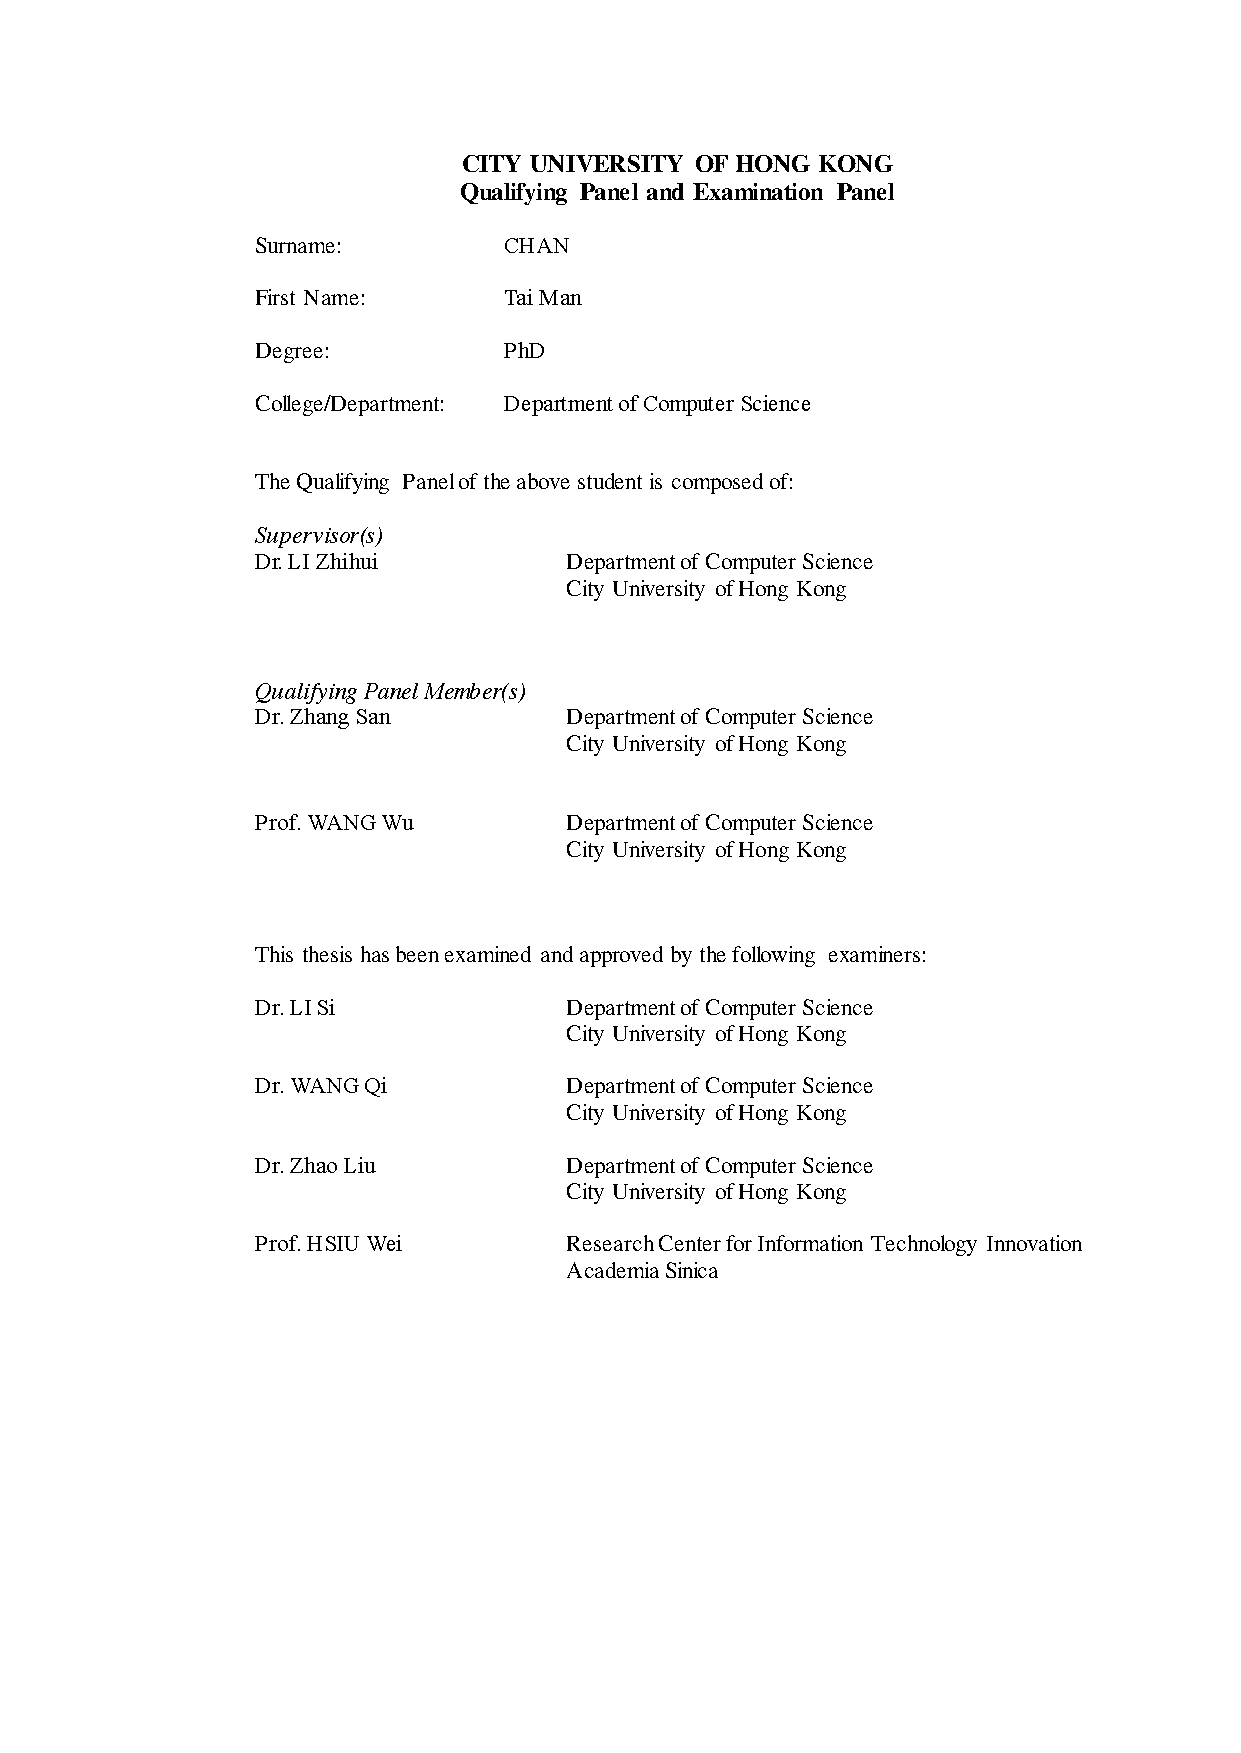
\includepdf[pagecommand={\thispagestyle{plain}}]{Front/qpsheet.pdf}

% Method 2:
% You may need to adjust the space to fit contents to one page
\begin{panel}

\begin{tabular}{p{40mm}p{80mm}}
Surname: & CHAN\tabularnewline
First Name: & Tai Man\tabularnewline
Degree: & PhD\tabularnewline
College/Department: & Department of Computer Science
\end{tabular}

\vspace{2em}

The Qualifying Panel of the above student is composed of:

\vspace{1em}

\begin{tabular}{p{50mm}p{80mm}}
\textit{Supervisor(s)} & \tabularnewline
Dr. SURNAME Name & Department of Computer Science\tabularnewline
 & City University of Hong Kong\\[1em]\tabularnewline

%\textit{Co-supervisor(s)} & \tabularnewline
%Name SURNAME & Department of ???\tabularnewline
% & City University of Hong Kong\\[.2em]\tabularnewline
 
\textit{Qualifying Panel Member(s)} & \tabularnewline
Prof. SURNAME Name & Department of Computer Science\tabularnewline
 & City University of Hong Kong\\[.2em]\tabularnewline

Dr. SURNAME Name & Department of Computer Science\tabularnewline
 & City University of Hong Kong\\[.2em]\tabularnewline
\end{tabular}

\vspace{2em}

This thesis has been examined and approved by the following examiners:
\vspace{1em}

\begin{tabular}{p{50mm}p{80mm}}
Prof. SURNAME Name & Department of Computer Science\tabularnewline
 & City University of Hong Kong\\[.2em]\tabularnewline

Dr. SURNAME Name & Department of Computer Science\tabularnewline
 & City University of Hong Kong\\[.2em]\tabularnewline

Prof. SURNAME Name & Department of Computer Science\tabularnewline
 & City University of Hong Kong\\[.2em]\tabularnewline

Dr. SURNAME Name & Department of Computer Science\tabularnewline
 & City University of Hong Kong\\[.2em]\tabularnewline
\end{tabular}

\end{panel}


% (d) Acknowledgment, if any
% ************************** Thesis Acknowledgements **************************
\begin{acknowledgements}
% \usepackage{parskip}
\setlength{\parindent}{0pt}

The path toward to the 'ACGN' has been circuitous. Its completion is thanks in large part to the special people who supported, assisted and accompanied to me along the way.

I would like to thank my dear friends-the seveners, who lead me to the fields by DeathNote, DNF, Naruto and Ge Ping. Their patient listening, unconditional help, warm company and sharing helped me to move forward better.

\lipsum[1-3]

\clearpage
\end{acknowledgements}


% (e) The table of contents and, where appropriate, a list of plates, tables, 
% figures, symbols or other abbreviations
% *********************** Adding TOC and List of Figures ***********************

\tableofcontents
% change the font size of \listoffigures, \listoftables
\chapternumberfont{\fontsize{20pt}{20pt}\selectfont}
\chaptertitlefont{\fontsize{17pt}{17pt}\selectfont}

% List of publications
%!TEX root = ../thesis.tex
% Author: Sankarea
%Date: 2022.05
% \usepackage{ulem}
%\usepackage{enumitem} %[leftmargin=*] Remove indent when using enumerate
\begin{publications}
\renewcommand{\ULthickness}{1.3pt} % thickness of underline
\noindent
\uline{\textbf{Paper Published ($^\dag{}$co-first author)}} % add dag
\begin{enumerate}[leftmargin=*]
\item \uline{\textbf{Yuzuriha Inori}}, Egoist, Chelly, Supercell, Ryo$^*$. Departures~Anata ni Okuru Ai no Uta~. \textit{Guilty Crown}. 2011 ; Vol. 1. \textbf{(IF=12.9)}

\item Kana Nishino$^\dag{}$, \uline{\textbf{Kanayan$^\dag{}$}}, Tookutemo ft. WISE, Always, Motto.., Kiminokoewo feat.Verbal(m-flo), SME Records$^*$, Sony Music Artists$^*$. Best friend: the first song of Kana I heared at highschool. \textit{First be Heared as BGM of a DNF video}. 2010 ; Vol. 2. \textbf{(IF=24)}
\end{enumerate}

\noindent
\uline{\textbf{Paper Forthcoming ($^\dag{}$co-first author)}}
\begin{enumerate}[leftmargin=*]
\item \uline{\textbf{Aikono Kikakina$^\dag{}$}}, Koeda$^\dag{}$, Black Rock Shooter, Sony Records, supercell$^*$, Ryo$^*$. My Desrest: So, everything that makes me whole. (Submitted, under review)
\end{enumerate}

\end{publications}

% List of  Abbreviations
% ************************** Thesis Abbreviations *****************************
% reference: https://tex.stackexchange.com/questions/4400/how-can-one-make-a-table-without-borders
% 自定义空格长度:https://juejin.cn/post/6933209801585328142

\begin{abbreviations}
% \begin{tabular}{lllll}
\begin{longtable}{@{\extracolsep{\fill}}lll@{}}
WuKe & \hspace{4em} & A bald man emerges from the crowd \\
Chief & & Wo Dao He Bei Sheng Lai \\
San Diego & &  50 meters NPK fertilize \\
Philosophy & & Banana Kun \\ %${\♂}$
 & &  \\
Death Note & & boku wa sinn sekai no kami to naru\\
Chobits & & Let Me Be With You \\
Fullmetal Alchemist & & LET IT OUT \\
Beelzebub & & Hildegarde \\
Madoka & & Puella Magi Madoka Magica \\
Silver Spoon & & Goose house \\
& &  \\
DNF & & Dungeon and Fighter \\
Danganronpa & & Trigger Happy Havoc \\
SteinsGate & & El Psy Kongroo \\
Air & & Jun Maeda \\
& &  \\
Youth Romantic Comedy & & My Youth Romantic Comedy \\
& & Is Wrong As I Expected \\
Durarara!! & & Trust Me \\
Rakkyo & & The Garden of Sinners \\
AW & & Accel World \\
& &  \\
CAFs & & Cancer-Associated Fibroblasts \\
CEA & & Carcinoembryonic Antigen \\
CDF & & Cumulative Distribution Function \\
CNN & & Convolutional Neural Network \\
CNV & & Copy Number Variant \\
CMS & &  Consensus Molecular Subtype \\
CRC & & Colorectal Cancer \\
CT & & Computed Tomography \\
CTx & & Adjuvant Chemotherapy \\
DFI & & Disease-Free Interval \\
DFS & & Disease-Free Survival \\
EAC & & Esophageal Adenocarcinoma \\
EC & & Esophageal Cancer \\
ECM & & Extracellular Matrix \\
EMT & & Epithelial-Mesenchymal Transition \\
ESCC & & Esophageal Squamous Cell Carcinoma \\
FDA & & U.S. Food and Drug Administration \\
OS & & Overall Survival \\
PCC & & Pearson Correlation Coefficient \\
px & & Pixels \\
RF & & Random Forests \\
RFS & & Relapse-Free Survival \\
ROC & & Receiver Operating Characteristic \\
% \end{tabular}
\end{longtable}
\clearpage
\end{abbreviations}

\listoffigures

\listoftables

% \printnomenclature[space] space can be set as 2em between symbol and description
%\printnomenclature[3em]

% \printnomenclature

% (f) The general text
% ******************************** Main Matter *********************************
\mainmatter

%!TEX root = ../thesis.tex
\chapternumberfont{\fontsize{20pt}{20pt}\selectfont}
\chaptertitlefont{\fontsize{18pt}{18pt}\selectfont}

\chapter{Mainly introduce the methods and changes of citation, figures, headers and table}
\chaptermark{Introduction} % shown as header

\section{Mainly introduce the citation methods}

\textbf{Here is the first citation \cite{1_GCS2020}.}


"Sanhua Remi" (Japanese:sankare, Hong Kong and Taiwan translation: "How can zombies be so cute?" ) is a comic book serialized by Japanese cartoonist Hattori in Kodansha 's comic magazine " Bessatsu Shonen Magazine ". finished. There are derivative works such as animation. 

\textbf{Here is the two to four citations \cite{2_CA, 3_PSM, 4_HUANG2014}.}

The manga "Sanhua Reiya" is a manga series serialized by Japanese manga artist Hattori Hattori in Kodansha's manga magazine "Bessatsu Shonen Magazine". The work tells the story of the protagonist, Chihiro Fukutani, who accidentally made the dead heroine Sanhua Reya become a zombie due to the resurrection technique. In order to maintain Reya's body and realize her desire to become an "ordinary girl" "The story of the desire to run hard. It was serialized in the January 2010 issue of Kodansha's magazine "Bessatsu Shonen Magazine", and its special chapters were also published in irregular issues in "Weekly Shonen Magazine". It ended in the October issue of Weekly Shonen Magazine, which was released in September 2014.


\textbf{\textit{Here is the last citations \cite{5_Huang2020, 6_Huang2019}.}}

\section[The example of setting headers with longlonglonglong title]{The example of setting headers with longlonglonglong title%
  \sectionmark{The example set to short}}
\sectionmark{The example set to short}

Lorem ipsum dolor sit amet, consectetuer adipiscing elit. Ut purus elit, vestibulum ut, placerat ac, adipiscing vitae, felis. Curabitur dictum gravida mauris. Nam arcu libero, nonummy eget, consectetuer id, vulputate a, magna. Donec vehicula augue eu neque. Pellentesque habitant morbi tristique senectus et ne-
tus et malesuada fames ac turpis egestas. Mauris ut leo. 

% Table 1 from picture or you could manually create tables as shown in table 1.2
\begin{table}[htbp!]
  \caption[The name which will be shown on TOC]{The Figure names and figure legends. \textbf{(a)} ahahda dqwe ead asd. \textbf{(b-d)} ahahda dqwe ead asd.}
  \centering
  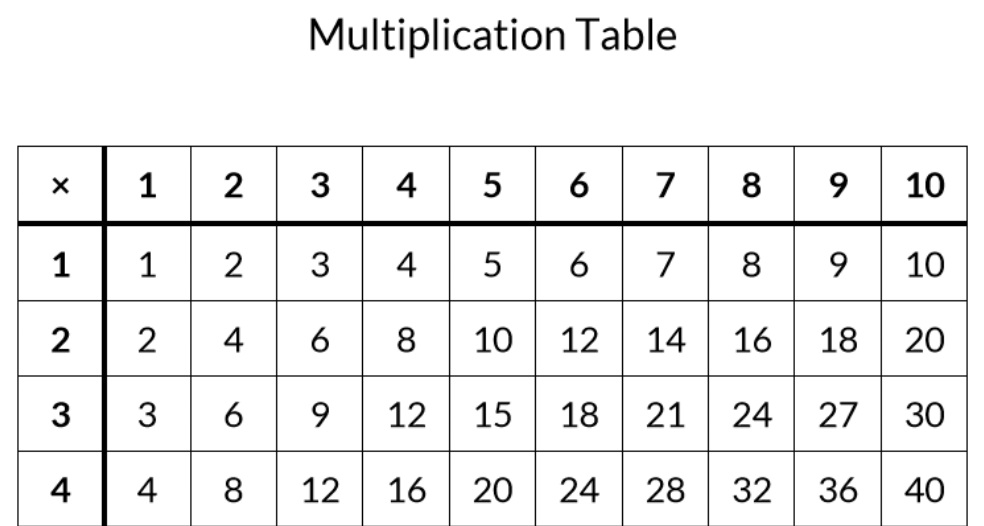
\includegraphics[width=1\textwidth]{Table 1.1} % the table figure name 
  % \label{tab1.1} not used here
\end{table}

\lipsum[1]

% Table 1.2
\begin{table}
\caption{Even better looking table using booktabs}
\centering
\label{table:good_table}
\begin{tabular}{l c c c c}
\toprule
\multirow{2}{*}{Dental measurement} & \multicolumn{2}{c}{Species I} & \multicolumn{2}{c}{Species II} \\
\cmidrule{2-5}
  & mean & SD  & mean & SD  \\
\midrule
I1MD & 6.23 & 0.91 & 5.2  & 0.7  \\

I1LL & 7.48 & 0.56 & 8.7  & 0.71 \\

I2MD & 3.99 & 0.63 & 4.22 & 0.54 \\

I2LL & 6.81 & 0.02 & 6.66 & 0.01 \\

CMD & 13.47 & 0.09 & 10.55 & 0.05 \\

CBL & 11.88 & 0.05 & 13.11 & 0.04\\
\bottomrule
\end{tabular}
\end{table}

% figure 1.1, the afterpage methods always put the figure at the top of new page.
\afterpage{
    \centering
    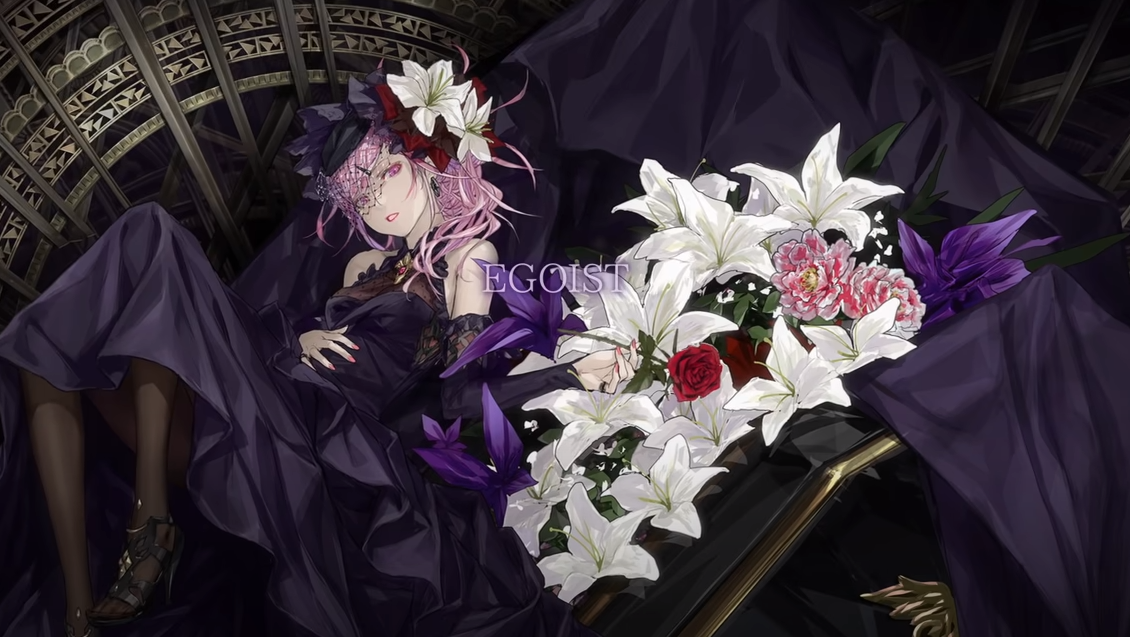
\includegraphics[width=1\textwidth]{Figure 1.1}
    \captionsetup{parbox=none}
    \captionof{figure}[Examples of something here to shown the afterpage figure methods.]{\textbf{Examples of something here to shown the afterpage figure methods.} \textbf{(a)} A hematoxylin and eosin (H{\&}E)-stained whole-slide image \textbf{(b)} Examples of something here to shown the afterpage figure methods. \textbf{(c)} Examples of something here to shown the afterpage figure methods.}
    % \vspace{\intextsep}
}

Lorem ipsum dolor sit amet, consectetuer adipiscing elit. Ut purus elit, vestibulum ut, placerat ac, adipiscing vitae, felis. Curabitur dictum gravida mauris. Nam arcu libero, nonummy eget, consectetuer id, vulputate a, magna. Donec vehicula augue eu neque. Pellentesque habitant morbi tristique senectus et ne-
tus et malesuada fames ac turpis egestas. Mauris ut leo. Lorem ipsum dolor sit amet, consectetuer adipiscing elit. Ut purus elit, vestibulum ut, placerat ac, adipiscing vitae, felis. Curabitur dictum gravida mauris. Nam arcu libero, nonummy eget, consectetuer id, vulputate a, magna. Donec vehicula augue eu neque. Pellentesque habitant morbi tristique senectus et netus et malesuada fames ac turpis egestas. Mauris ut leo. Lorem ipsum dolor sit amet, consectetuer adipiscing elit. Ut purus elit, vestibulum ut, placerat ac, adipiscing vitae, felis. Curabitur dictum gravida mauris. Nam arcu libero, nonummy eget, consectetuer id, vulputate a, magna. Donec vehicula augue eu neque. Pellentesque habitant morbi tristique senectus et netus et malesuada fames ac turpis egestas. Mauris ut leo. Lorem ipsum dolor sit amet, consectetuer adipiscing elit. Ut purus elit, vestibulum ut, placerat ac, adipiscing vitae, felis. Curabitur dictum gravida mauris. Nam arcu libero, nonummy eget, consectetuer id, vulputate a, magna. Donec vehicula augue eu neque. Pellentesque habitant morbi tristique senectus et netus et malesuada fames ac turpis egestas. Mauris ut leo.

% Figure 1.2  the begin{figure} method could put into any place if the space is enough on the current page.
\begin{figure}[htbp!]
  \centering
  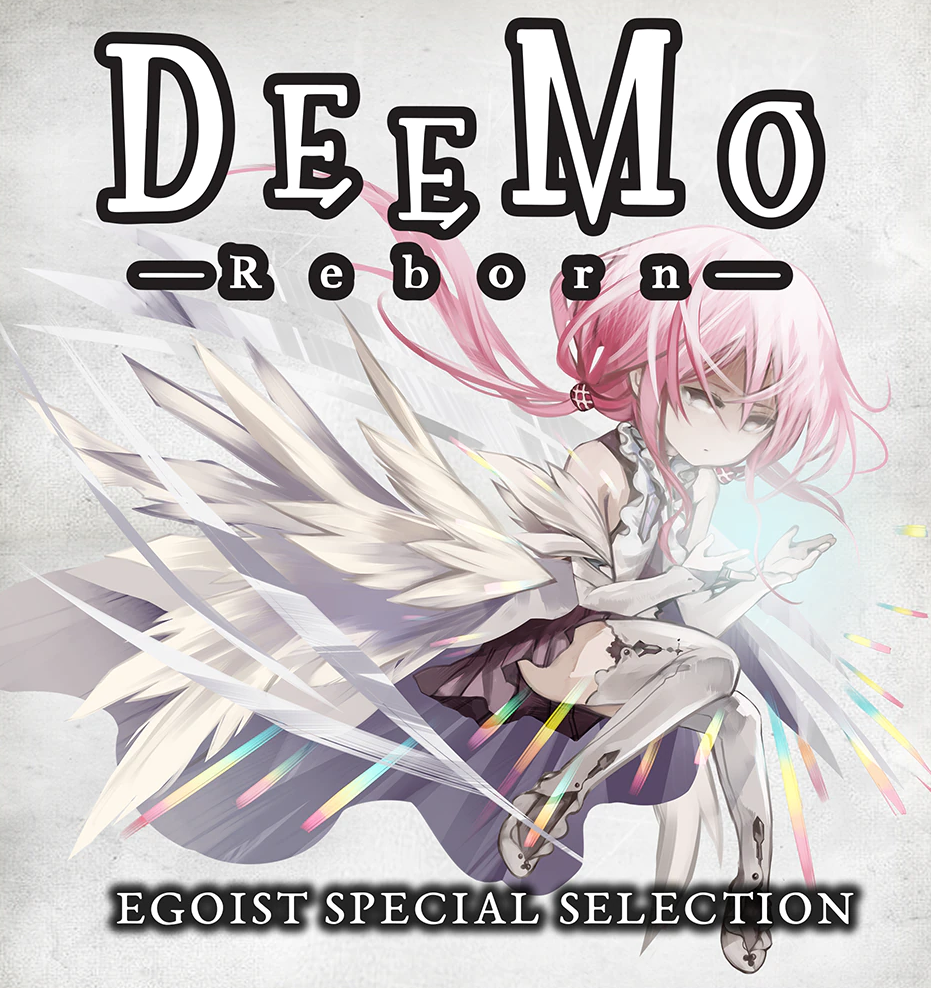
\includegraphics[width=0.7\textwidth]{Figure 1.2}
  \caption[the begin{figure} method could put into any place if the space is enough on the current page.]{\textbf{the begin{figure} method could put into any place if the space is enough on the current page. But figure 1.2 did not have the enough space to put on the current pages.} the begin{figure} method could put into any place if the space is enough on the current page. But figure 1.2 did not have the enough space to put on the current pages. the begin{figure} method could put into any place if the space is enough on the current page.the begin{figure} method could put into any place if the space is enough on the current page.the begin{figure} method could put into any place if the space is enough on the current page.}
  \end{figure}


\section{Objectives of the Study}

The overall goal of this study is to dissect and further investigate the association with  based on . 

An efficient and robust Comic framework is proposed to dissect the purity of users. The detailed description and results of our exploration will be introduced in \textbf{Chapter 2}.


Next, a deep learning framework-Game Center is designed for fully automated user classification through transfer learning from Anime. Our exploration will be detailed in \textbf{Chapter 3}.


The multi-omics Novel subtyping is translated into the clinic by developing a light novel classification system. These interesting studies will be discussed in \textbf{Chapter 4}.


% Figure 1.2  the begin{figure} method could put into any place if the space is enough on the current page.
\begin{figure}[htbp!]
  \centering
  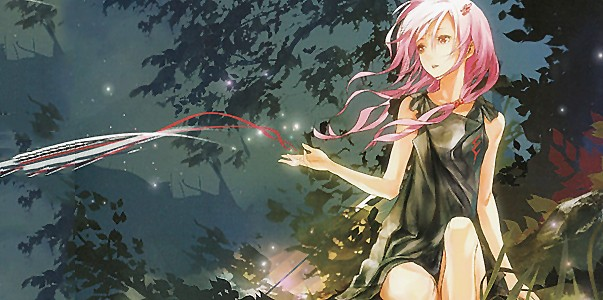
\includegraphics[width=1\textwidth]{Figure 1.3}
  \caption[But figure 1.2 did not have the enough space to put on the current pages]{\textbf{the begin{figure} method could put into any place if the space is enough on the current page.}}
  \end{figure}



\section{Thesis outline}

\begin{itemize}
    \item \textbf{Chapter1:} Introduction to .
    \item \textbf{Chapter2:} Identification of in Microenvironment using Deep Learning.
    \item \textbf{Chapter3:} Deep Learning-derived analysis on .
    \item \textbf{Chapter4:} Multi-Omics Novel subtyping of light novel using Deep Learning.
    \item \textbf{Chapter5:} Conclusion and Future Prospective.
\end{itemize}

%!TEX root = ../thesis.tex
% 注意p,test斜体,Figure, Table加粗 123
\chapternumberfont{\fontsize{20pt}{20pt}\selectfont}
\chaptertitlefont{\fontsize{18pt}{18pt}\selectfont}

\chapter{Extra chapter for presentation of formula, table of content}
\chaptermark{Extra presentation}

Some background here.

\section{INTRODUCTION} %section

Lorem ipsum dolor sit amet, consectetuer adipiscing elit. Ut purus elit, vestibulum ut, placerat ac, adipiscing vitae, felis. Curabitur dictum gravida mauris. Nam arcu libero, nonummy eget, consectetuer id, vulputate a, magna. Donec vehicula augue eu neque. Pellentesque habitant morbi tristique senectus et ne-
tus et malesuada fames ac turpis egestas. Mauris ut leo.

\section{MATERIALS AND METHODS} %section
\subsection{The math formula} %section

\textbf{there are online tools for the latex version of math formula}:

\begin{equation}
  \centering
  WCDI_A = \frac{1}{n_A} {\textstyle \sum_{i\in A}^{}}\frac{1}{n_{A_i}}   {\textstyle \sum_{j\in A_i}^{}}d(i, j)
  \end{equation}  

Lorem ipsum dolor sit amet, consectetuer adipiscing elit. Ut purus elit, vestibulum ut, placerat ac, adipiscing vitae, felis. Curabitur dictum gravida mauris. Nam arcu libero, nonummy eget, consectetuer id, vulputate a, magna. Donec vehicula augue eu neque. Pellentesque habitant morbi tristique senectus et ne-tus et malesuada fames ac turpis egestas. Mauris ut leo.

\begin{equation}
  \centering
  WCDI_A = \frac{1}{n_A} {\textstyle \sum_{i\in A}^{}}\frac{1}{n_{A_i}}   {\textstyle \sum_{j\in A_i}^{}}d(i, j)
  \end{equation} 

\subsection{Statistical Analysis} %2.2.6

Statistical analysis was conducted with R software (version 3.6.1; http://www.R\\project.org). Descriptive statistics were computed for all variables, including means and standard deviations (SD) or medians and frequencies for categorical factors. Continuous values were compared using Wilcoxon Signed-rank tests between different groups. A \textit{p}-value of less than 0.05 was considered statistically significant in all tests.

\section{RESULTS} %section
\subsection{abababababab balalala whowhowhowho wuhuwuhuwuhu} %section

Lorem ipsum dolor sit amet, consectetuer adipiscing elit. Ut purus elit, vestibulum ut, placerat ac, adipiscing vitae, felis. Curabitur dictum gravida mauris. Nam arcu libero, nonummy eget, consectetuer id, vulputate a, magna. Donec vehicula augue eu neque. Pellentesque habitant morbi tristique senectus et ne-
tus et malesuada fames ac turpis egestas. Mauris ut leo.

\subsection{whowhowhowho wuhuwuhuwuhu abababababab balalala } %section

Lorem ipsum dolor sit amet, consectetuer adipiscing elit. Ut purus elit, vestibulum ut, placerat ac, adipiscing vitae, felis. Curabitur dictum gravida mauris. Nam arcu libero, nonummy eget, consectetuer id, vulputate a, magna. Donec vehicula augue eu neque. Pellentesque habitant morbi tristique senectus et ne-
tus et malesuada fames ac turpis egestas. Mauris ut leo.




% ********************************** Back Matter *******************************
% Backmatter should be commented out, if you are using appendices after References
% \backmatter

% (g) Bibliography
% ********************************** Bibliography ******************************
\begin{spacing}{0.9}

% To use the conventional natbib style referencing
\nocite{*}
% \bibliographystyle{apalike} # used for duplicate check
% \bibliographystyle{ieeetran} % not IEEEtran
\bibliographystyle{unsrt} % Use for unsorted references
% \bibliographystyle{plainnat} % use this to have URLs listed in References
\cleardoublepage
\bibliography{References/references} % Path to your References.bib file


% If you would like to use BibLaTeX for your references, pass `custombib' as
% an option in the document class. The location of 'reference.bib' should be
% specified in the preamble.tex file in the custombib section.
% Comment out the lines related to natbib above and uncomment the following line.

% \printbibliography[heading=bibintoc, title={References}]

\end{spacing}

% (h) Appendices and other addenda, if any.
% ********************************** Appendices ********************************

\begin{appendices} % Using appendices environment for more functunality
% \renewcommand\chaptername{APPENDIX}
%!TEX root = ../thesis.tex

% the table could be created from excel by online tools:
% https://tableconvert.com/csv-to-latex
% https://www.tablesgenerator.com/

\chapternumberfont{\fontsize{16pt}{16pt}\selectfont}
\chaptertitlefont{\fontsize{16pt}{16pt}\selectfont}

\chapter{The example based on project of Instrumentality of Mankind}
\chaptermark{Project of Instrumentality of Mankind}

\setlength\LTleft{0pt}
\setlength\LTright{0pt}
\begin{longtable}{@{\extracolsep{\fill}}lll@{}}
% 竖线边界由 |c|c|c| 或者\cline 决定,没有|||,则没有border
    \toprule  % 粗上线
    \multicolumn{1}{l}{\textbf{Subtypes}} & \textbf{Features}                   & \textit{\textbf{P}} \\ \hline
    \endhead % add title for each page
                                          & index\_1                            & 1.87E-18            \\
                                          & index\_1                            & 1.87E-18            \\
                                          & index\_1                            & 1.87E-18            \\
                                          & index\_1                            & 1.87E-18            \\
                                          & index\_1                            & 1.87E-18            \\
                                          & index\_1                            & 1.87E-18            \\
                                          & index\_1                            & 1.87E-18            \\
\textbf{Subtypeee1}                       & index\_1                            & 1.87E-18            \\
                                          & index\_1                            & 1.87E-18            \\
                                          & index\_1                            & 1.87E-18            \\
                                          & index\_1                            & 1.87E-18            \\
                                          & index\_1                            & 1.87E-18            \\
                                          & index\_1                            & 1.87E-18            \\
                                          & index\_1                            & 1.87E-18            \\
                                          & index\_1                            & 1.87E-18            \\
                                          & index\_1                            & 1.87E-18            \\
                                          \hline % manually set the bottom line on each page end
                                          & index\_1                            & 1.87E-18            \\
                                          & index\_1                            & 1.87E-18            \\
                                          & index\_1                            & 1.87E-18            \\
                                          & index\_1                            & 1.87E-18            \\
                                          & index\_1                            & 1.87E-18            \\
                                          & index\_1                            & 1.87E-18            \\
                                          & index\_1                            & 1.87E-18            \\
\textbf{Subtypeee1}                       & index\_1                            & 1.87E-18            \\
                                          & index\_1                            & 1.87E-18            \\
                                          & index\_1                            & 1.87E-18            \\
                                          & index\_1                            & 1.87E-18            \\
                                          & index\_1                            & 1.87E-18            \\
                                          & index\_1                            & 1.87E-18            \\
                                          & index\_1                            & 1.87E-18            \\
                                          & index\_1                            & 1.87E-18            \\
                                          & index\_1                            & 1.87E-18            \\
                                          \hline
                                          & index\_1                            & 1.87E-18            \\
                                          & index\_1                            & 1.87E-18            \\
                                          & index\_1                            & 1.87E-18            \\
                                          & index\_1                            & 1.87E-18            \\
\textbf{Subtypeee2}                       & index\_1                            & 1.87E-18            \\
                                          & index\_1                            & 1.87E-18            \\
                                          & index\_1                            & 1.87E-18            \\
                                          & index\_1                            & 1.87E-18            \\
                                          & index\_1                            & 1.87E-18            \\
                                          & index\_1                            & 1.87E-18            \\
                                          \hline
                                          & index\_1                            & 1.87E-18            \\
                                          & index\_1                            & 1.87E-18            \\
                                          & index\_1                            & 1.87E-18            \\
                                          & index\_1                            & 1.87E-18            \\
                                          & index\_1                            & 1.87E-18            \\
                                          & index\_1                            & 1.87E-18            \\
                                          & index\_1                            & 1.87E-18            \\
\textbf{Subtypeee3}                       & index\_1                            & 1.87E-18            \\
                                          & index\_1                            & 1.87E-18            \\
                                          & index\_1                            & 1.87E-18            \\
                                          & index\_1                            & 1.87E-18            \\
                                          & index\_1                            & 1.87E-18            \\
                                          & index\_1                            & 1.87E-18            \\
                                          \bottomrule

\end{longtable}
\end{appendices}

\end{document}
 